

% STRIDE Chapter: Expanded and Enhanced
\subsection*{1. Introduction to STRIDE}
STRIDE is a foundational threat modeling framework developed by Microsoft to help security professionals systematically identify and categorize threats in software systems\cite{shostack2014}. The acronym stands for Spoofing, Tampering, Repudiation, Information Disclosure, Denial of Service, and Elevation of Privilege. Each category represents a distinct type of threat that can undermine the confidentiality, integrity, or availability of a system. By breaking down threats into these six categories, STRIDE enables teams to analyze every component and data flow within an application, ensuring that no potential risk is overlooked.

\subsection*{2. Technical Definitions and Real-World Examples}
The STRIDE framework provides clear definitions and practical examples for each threat category:
\begin{itemize}
	\item \textbf{Spoofing:} Pretending to be someone or something else to gain unauthorized access. Example: Attackers use stolen credentials or exploit weak authentication mechanisms to impersonate legitimate users\cite{shostack2014}. Spoofing undermines trust and can lead to further compromise of sensitive data and systems.
	\item \textbf{Tampering:} Unauthorized modification of data or code, such as altering database records via SQL injection or manipulating configuration files\cite{owasp}. Tampering can disrupt operations, corrupt data, and facilitate additional attacks.
	\item \textbf{Repudiation:} The ability of users to deny their actions, often due to insufficient logging or lack of digital signatures\cite{nist800154}. Repudiation complicates incident response and forensic investigations, making it difficult to hold malicious actors accountable.
	\item \textbf{Information Disclosure:} Accidental or malicious exposure of confidential data, such as leaking personally identifiable information (PII) through misconfigured APIs or insecure storage\cite{uceda2015}. Information disclosure can result in regulatory penalties, reputational damage, and loss of customer trust.
	\item \textbf{Denial of Service:} Attacks that disrupt the availability of a service, such as distributed denial-of-service (DDoS) attacks targeting login endpoints or critical infrastructure\cite{owasp}. Denial of service can cause significant financial losses and operational downtime.
	\item \textbf{Elevation of Privilege:} Exploiting vulnerabilities to gain higher access rights than intended, such as leveraging a vulnerable admin panel to obtain root privileges\cite{shostack2014}. Elevation of privilege can lead to complete system compromise and persistent attacker presence.
\end{itemize}

\subsection*{3. STRIDE Threat Categories Table}
The following table summarizes the STRIDE categories, providing descriptions, examples, and recommended controls:
\begin{table}[H]
\centering
\begin{tabular}{|l|l|l|l|}
\hline
		extbf{Category} & \textbf{Description} & \textbf{Example} & \textbf{Control} \\
\hline
Spoofing & Impersonating users or systems & Stolen credentials & MFA, strong authentication \\
Tampering & Modifying data or code & SQL injection & Input validation, hashing \\
Repudiation & Denying actions & Log deletion & Audit logs, digital signatures \\
Information Disclosure & Leaking sensitive data & Data breach & Encryption, access control \\
Denial of Service & Disrupting service & DDoS attack & Rate limiting, WAF \\
Elevation of Privilege & Gaining unauthorized access & Privilege escalation & RBAC, least privilege \\
\hline
\end{tabular}
\caption{STRIDE Threat Categories, Examples, and Controls\cite{shostack2014,owasp}}
\end{table}

\subsection*{4. STRIDE and Data Flow Diagrams (DFDs)}
STRIDE is most effective when applied to Data Flow Diagrams (DFDs), which visually represent system components, data stores, and trust boundaries. By analyzing each element for threats in all STRIDE categories, security teams can systematically identify and address risks throughout the system\cite{shostack2014}. This approach ensures comprehensive coverage and supports the design of layered defenses.

\begin{figure}[H]
	\centering
	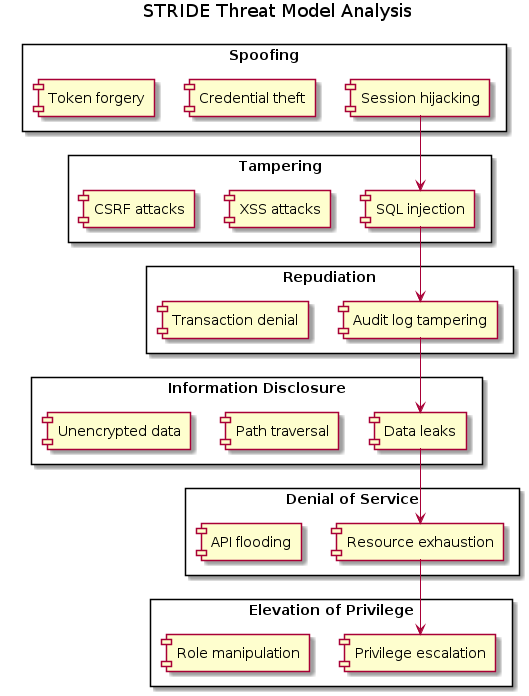
\includegraphics[width=0.7\textwidth]{images/stride-analysis}
	\caption{Example STRIDE Analysis on a Data Flow Diagram}
\end{figure}

\subsection*{5. Practical Application: STRIDE in Action}
To illustrate the application of STRIDE, consider a web application with user authentication, a database, and an admin panel. Security teams would analyze each component as follows:
\begin{itemize}
	\item \textbf{Spoofing:} Attackers use phishing or credential stuffing to impersonate users, bypassing authentication controls.
	\item \textbf{Tampering:} SQL injection attacks are used to alter database records, compromising data integrity.
	\item \textbf{Repudiation:} Malicious users delete logs to hide unauthorized actions, complicating incident response.
	\item \textbf{Information Disclosure:} Sensitive data is exposed through misconfigured APIs or insecure storage mechanisms.
	\item \textbf{Denial of Service:} Attackers flood the login endpoint, rendering the application unavailable to legitimate users.
	\item \textbf{Elevation of Privilege:} Exploiting vulnerabilities in the admin panel allows attackers to gain root access and control the system.
\end{itemize}

\subsection*{6. STRIDE in Secure Development}
Microsoft recommends integrating STRIDE into the Secure Development Lifecycle (SDL), using it to drive security requirements, code reviews, and testing. Modern tools, such as the Microsoft Threat Modeling Tool, automate parts of the STRIDE process and help teams visualize threats and mitigations\cite{shostack2014,owasp}. STRIDE’s structured approach is referenced in leading books and standards, including Shostack\cite{shostack2014}, UcedaVélez and Morana\cite{uceda2015}, and NIST SP 800-154\cite{nist800154}.

\subsection*{7. Academic Perspective and Further Reading}
STRIDE’s impact on the field is well documented in academic literature and industry practice. For deeper understanding, refer to:
\begin{itemize}
	\item Adam Shostack, "Threat Modeling: Designing for Security" (Wiley, 2014)
	\item Tony UcedaVélez and Marco M. Morana, "Risk Centric Threat Modeling" (Wiley, 2015)
	\item NIST SP 800-154: Guide to Data-Centric System Threat Modeling
	\item OWASP Threat Modeling Cheat Sheet
\end{itemize}
